\documentclass[12pt,a4paper]{article}
\usepackage{amsmath}
\usepackage{mathtext}
\usepackage{icomma}
\usepackage{amsfonts}
\usepackage{amssymb}
\usepackage[utf8]{inputenc}
\usepackage[T1,T2A]{fontenc}
\usepackage[english, russian]{babel}
\usepackage{graphicx}
\usepackage[left=2cm,right=2cm,top=2cm,bottom=2cm]{geometry}
\usepackage{calc}
\usepackage{wrapfig}
\usepackage{setspace}
\usepackage{indentfirst}
\usepackage{subfigure}
\usepackage[table,xcdraw]{xcolor}
\usepackage{float}

\title{Отчет о выполнении лабораторной работы 3.4.5\\
Резонанс напряжений}

\author{Исламов Сардор, группа Б02-111}
\date{29 октября 2022 г.}

\begin{document}
\maketitle
\subparagraph*{Аннотация.} 
В данной работе исследован резонанс напряжений в последовательном колебательном контуре с изменяемой ёмкостью, также исследован закон Ома.

\subsection*{Теоретическое введение}
Магнитную индукцию удобно определять с помощью ЭДС, возникающей при изменении потока в катушке, намотанной на образец. 
Пусть катушка плотно обхватывает образец, а индукция $\vec{B}$ однородна. 
Тогда
\[
\varepsilon = -\dfrac{d\Phi}{dt}, \Phi = BSN_\text{и} \Rightarrow |B|=\dfrac{1}{SN_\text{и}}\int \varepsilon dt,
\]
где $N_\text{и}$ -- число витков в измерительной катушке, $S$ -- площадь витка. 
То есть для определения $B$ нужно проинтегрировать сигнал, наведённый на измерительную катушку.\\
Используя интегрирующую схему из конденсатора $C$ опротивления $R \gg \dfrac{1}{\Omega C}$ ($\Omega$ -- частота сигнала в сети), с учётом $U_{\text{вых}} \ll U_{\text{вх}}$, получим
\[
U_{\text{вых}}=\dfrac{1}{C}\int Idt \approx \dfrac{1}{RC}\int U_{\text{вх}}dt
\]
Если $R_{\text{и}}$ и $C_{\text{и}}$ -- параметры интегрирующей ячейки, то получим
\begin{equation}
    |B| = \dfrac{R_{\text{и}}C_{\text{и}}}{SN_\text{и}}U_{\text{вых}} 
\end{equation}

\subsection*{Экспериментальная установка}
Схема установки представлена на рис. 1. 
\begin{figure}
    \centering
    \includegraphics*[width=0.8\linewidth]{pics/scheme.png}
    \caption{Схема установки для исследования намагничивания образцов}
\end{figure}
Напряжение сети с помощью регулировочного трансформатора Ат через разделительный понижающий трансформатор Тр подаётся на намагничивающую обмотку $N_0$ образца. 
Значение тока в обмотке измеряется амперметром А, с ним последовательно сопротивление $R_0$, напряжение с которого подается на вход Х электронного осциллографа (ЭО). 
Это напряжение пропорционально току в обмотке $N_0$, а значит и напряжённости магнитного поля $H$ в образце.\\
Для измерения магнитной индукции $B$ в обмотке $N_\text{и}$ на вход интегрирующей цепочки подаётся напряжение $U_\text{и}$, пропорциональное $\dfrac{dB}{dt}$, а с выхода снимается напряжение $U_C$, пропорциональное $B$, которое подаётся на вход Y ЭО.\\
Кривая, возникающая на экране, воспроизводит петлю гистерезиса. 
По формулам 
\[
H = \dfrac{IN_0}{2\pi R}, B = \dfrac{R_\text{и} C_\text{и}U_\text{вых}}{SN_\text{и}}
\]
где $I = K_X/R_0, U_\text{вых} = K_Y$, $K_X, K_Y$ -- чувствительность усилителя ЭФ соответствующих шкал, можно провести калиброку ЭО.\\
При закороченной обмотке $N_0$ амперметр измеряет эффективное значение синусоидального тока $I_\text{эф}$ через сопротивление $R_0$. Если $2x$ -- длина горизонтальной прямой на экране, то чувствительность канала Х
\begin{equation}
    m_X = \dfrac{2\sqrt{2}R_0I_\text{эф}}{2x}
\end{equation}
При отключённом тороиде сигнал с обмотки 12.6 В подаётся на делитель, и его часть снимается с делителя с каоэффициетном деления и подаётся на Y ЭО вместо $U_C$. Вольтметр измеряет напряжение $U_\text{эф}$ на этих клеммах делителя. Если $2y$ -- длина вертикальной прямой на экране, то чувствительность канал Y
\begin{equation}
    m_Y = \dfrac{2\sqrt{2}U_\text{эф}}{2y}
\end{equation}
Если измерить с помощью ЭО поочерёдно амлитуды сигналов $U_\text{вх}$ и $U_\text{вых}$ $RC$-цепочки, можно рассчитать постоянную времени 
\begin{equation}
    \tau = RC = \dfrac{U_\text{вх}}{\Omega U_\text{вых}}     
\end{equation}



\subsection*{Результаты измерений и обработка данных}
Для наблюдения петли гистерезиса на экране ЭО соберем схему согласно рис. 1, установим автотрансформатор на минимальное выходное напряжение.
Подберем коэффициенты усиления каналов ЭО так, чтобы предельная петля занимала большую часть экрана.

На рис. 2 изображены предельный петли гистерезиса для различних образцов, в табл. 1 их параметры.


\begin{figure}[H]
	\centering	
	\begin{minipage}{0.33\linewidth}
		\centering
		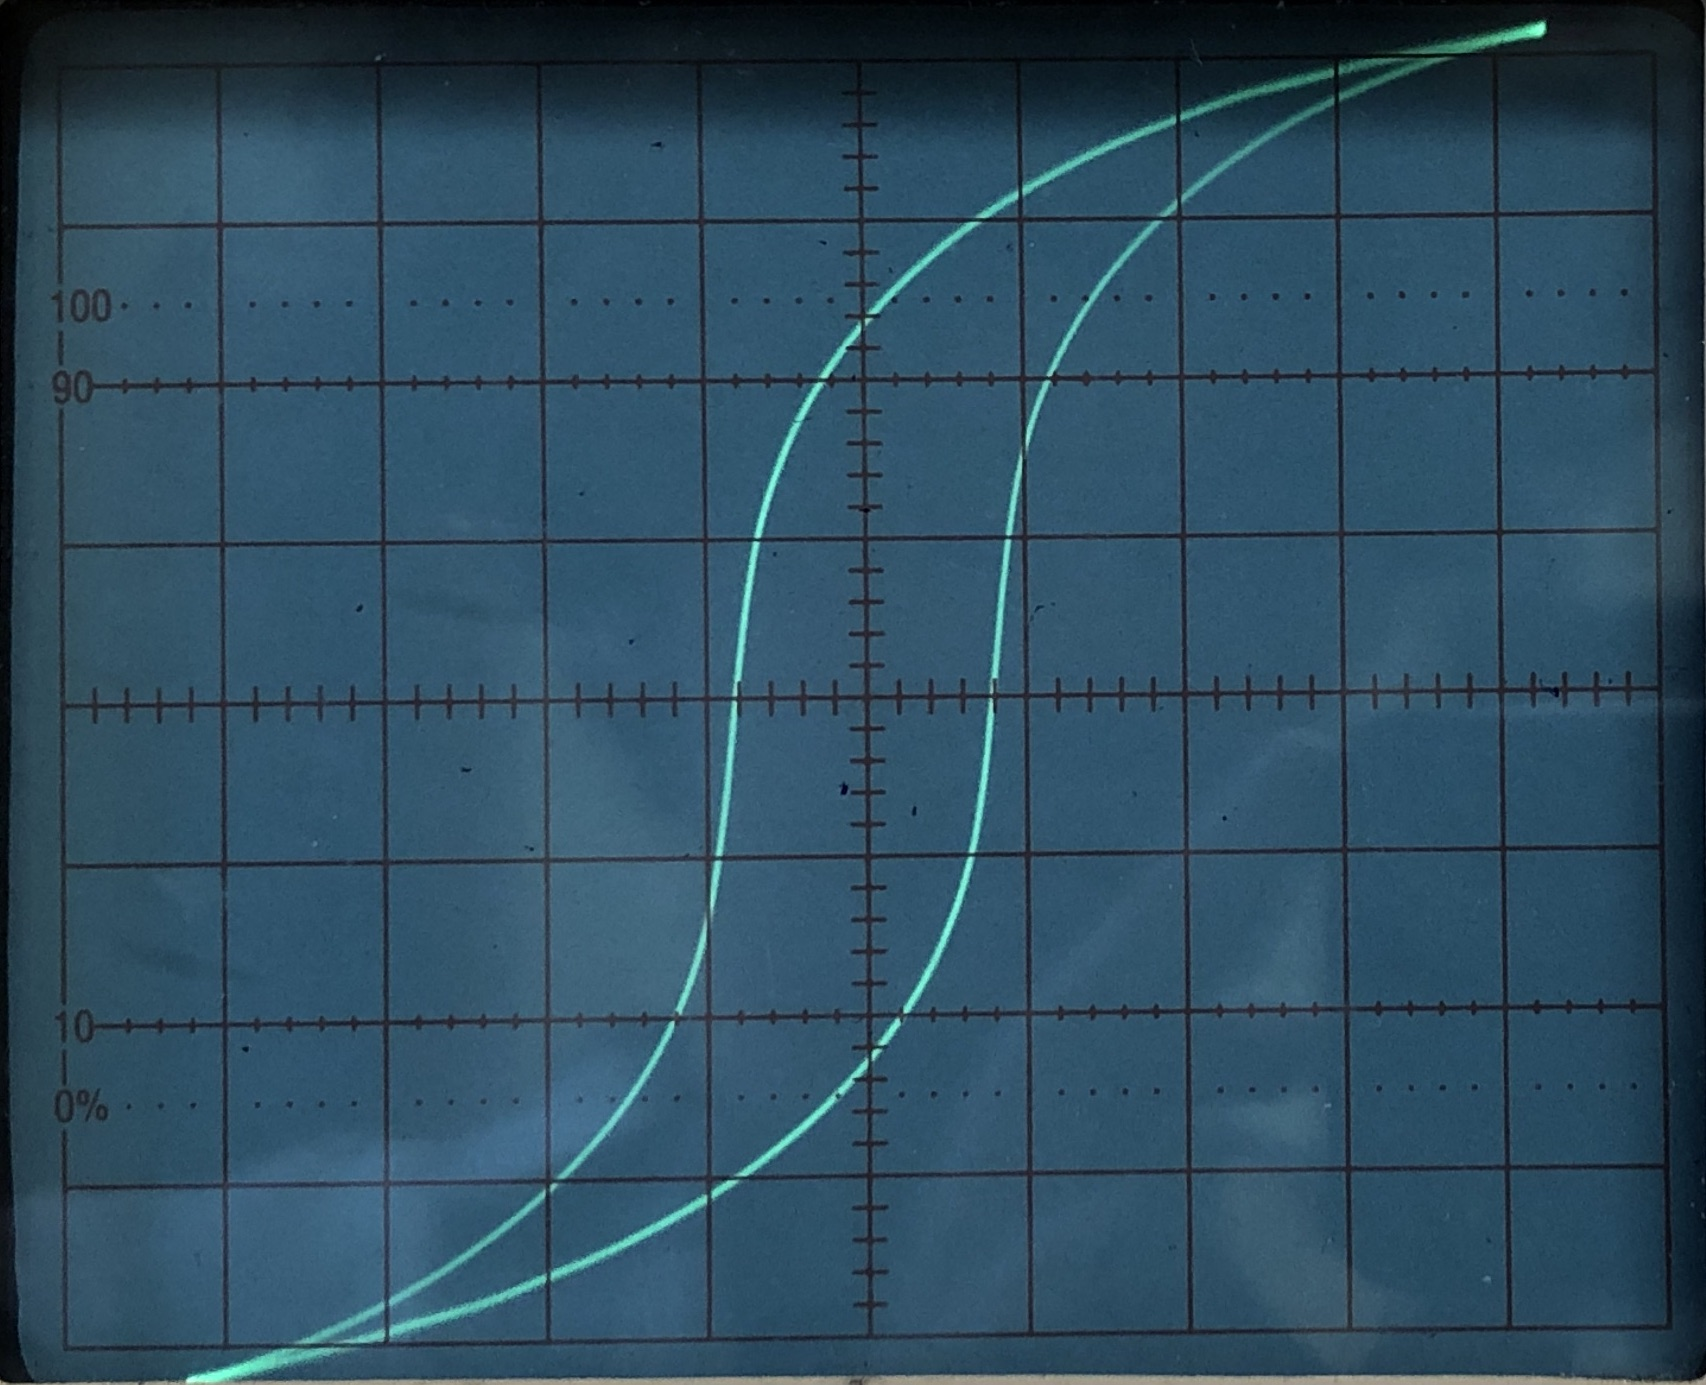
\includegraphics[width=0.9\linewidth]{pics/pred_ferrit.JPG}
		(a) Феррит
	\end{minipage}
	\begin{minipage}{0.33\linewidth}
		\centering
		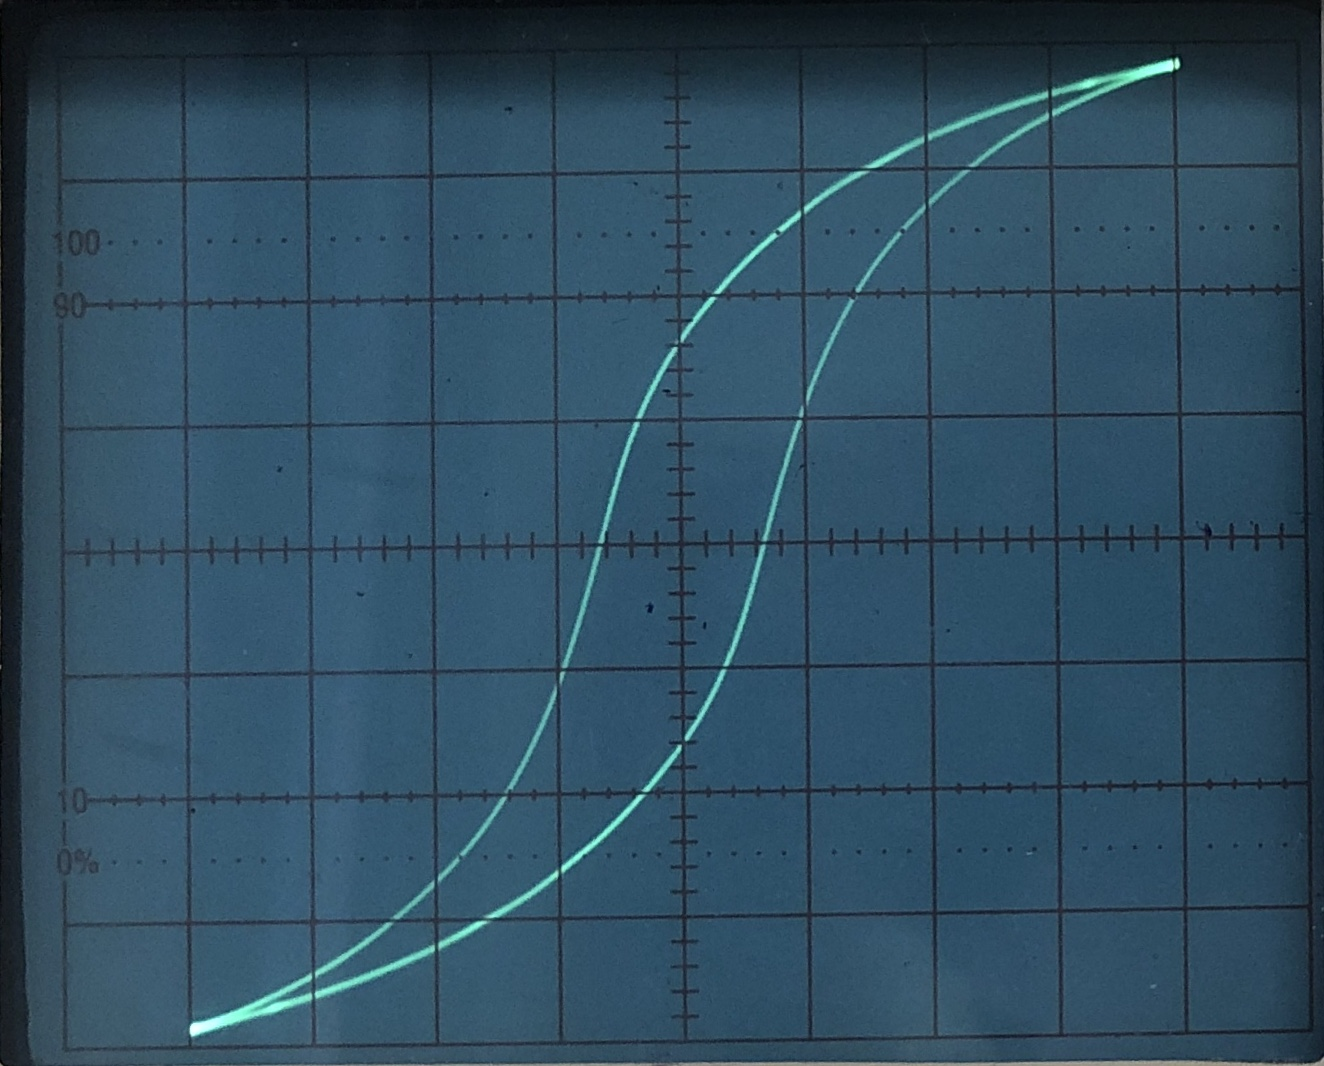
\includegraphics[width=0.9\linewidth]{pics/pred_sife.jpg}
		(б) Кремнистое железо
	\end{minipage}

	\begin{minipage}{0.33\linewidth}
		\centering
		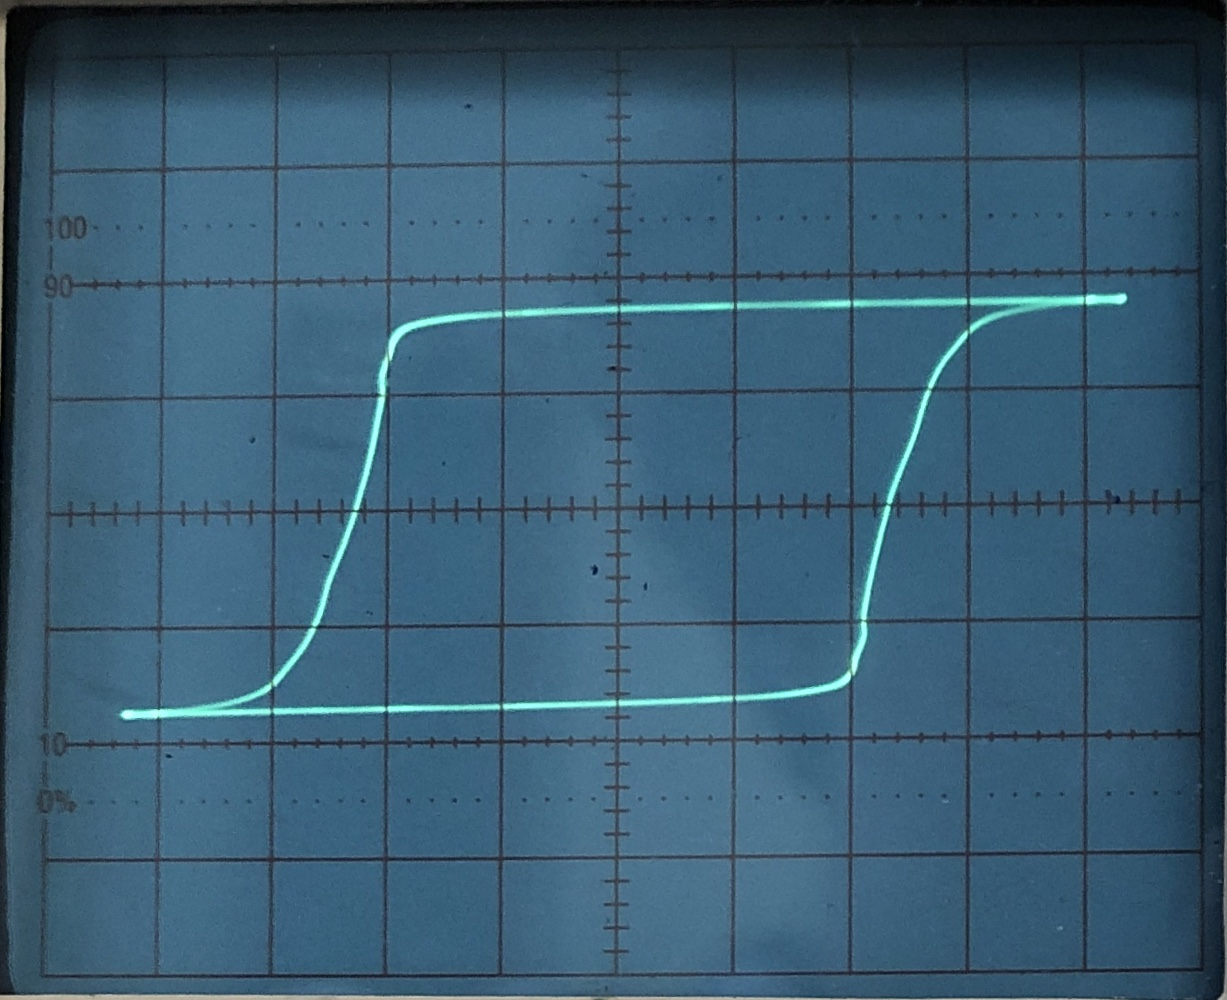
\includegraphics[width=0.9\linewidth]{pics/pred_perm.jpg}
		(в) Пермаллой
	\end{minipage}

	\caption{Предельные петли гистерезиса}
\end{figure}

\begin{table}[H]
    \centering
    \begin{tabular}[]{|l|c|c|c|}
        \hline
        &Феррит&Кремнистое железо&Пермаллой \\ \hline
        $N_0$ &45&20&15 \\ \hline
        $N_U$ &400&200&300 \\ \hline
        $S,\ см^2$ &3.0&2&0.66 \\ \hline
        $2\pi R,\ см$ &25&11&14.1 \\ \hline
    \end{tabular}
    \caption{Параметры образцов}
\end{table}

\begin{table}[H]
    \centering
    \begin{tabular}[]{|l|c|}
        \hline
        $R_0$ &0.2 Ом\\ \hline
        $R_и$ &20 кОм \\ \hline
        $C_и$ &20 мкФ\\ \hline
        $\Omega$ &50 Гц \\ \hline
    \end{tabular}
    \caption{Параметры установки}
\end{table}

Расчитаем цены деления $H = \dfrac{K_xN_0}{2\pi R R_0}$ и $B = \dfrac{R_и C_и K_у}{S N_U}$

\begin{table}[H]
    \centering
    \begin{tabular}[]{|l|c|c|c|}
        \hline
        &Феррит&Кремнистое железо&Пермаллой \\ \hline
        $H$, $\frac{А}{м\ дел}$ &9.0 &90.9&10.6 \\ \hline
        $B$, Тл/дел &0.033 &0.20 &1.01 \\ \hline
    \end{tabular}
    \caption{Цены деления}
\end{table}

По снятым показаниям для каждого образца восстановим начальную кривую намагничивания (рис. 3).

\begin{figure}[H]
	\centering	

    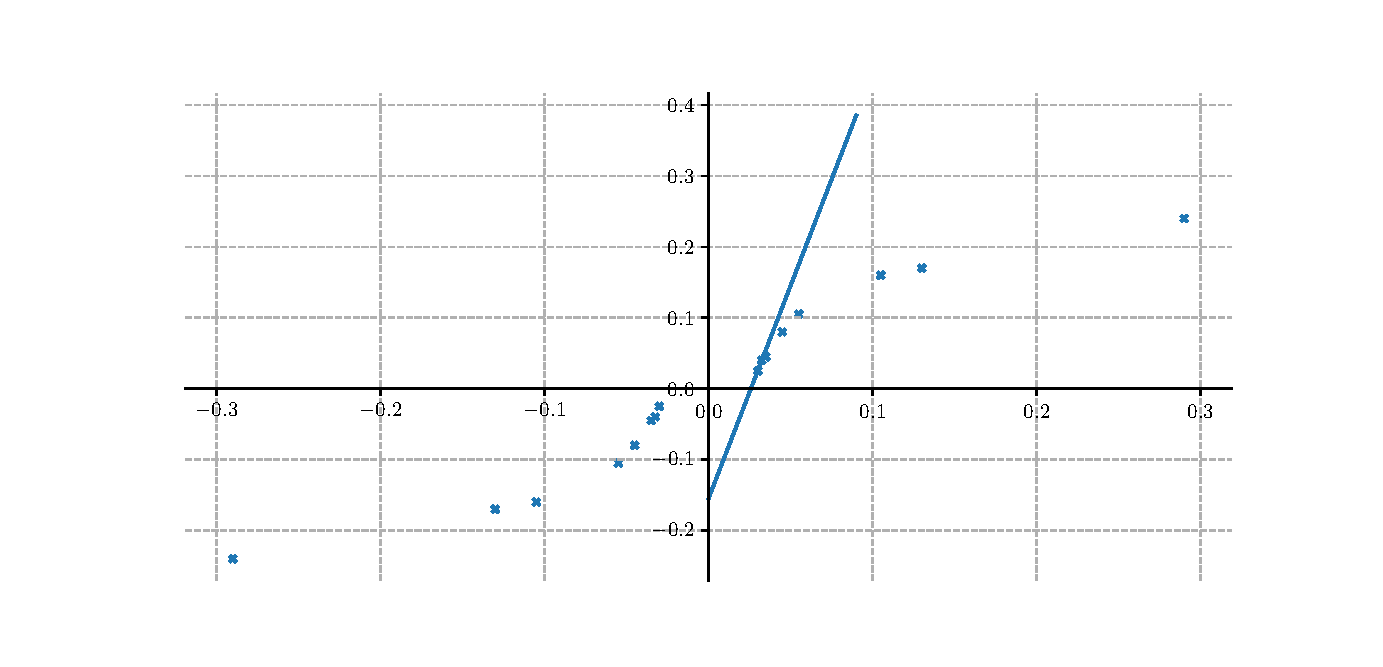
\includegraphics[width=0.9\linewidth]{pics/ferr.eps}
    \text{(a) Феррит}
    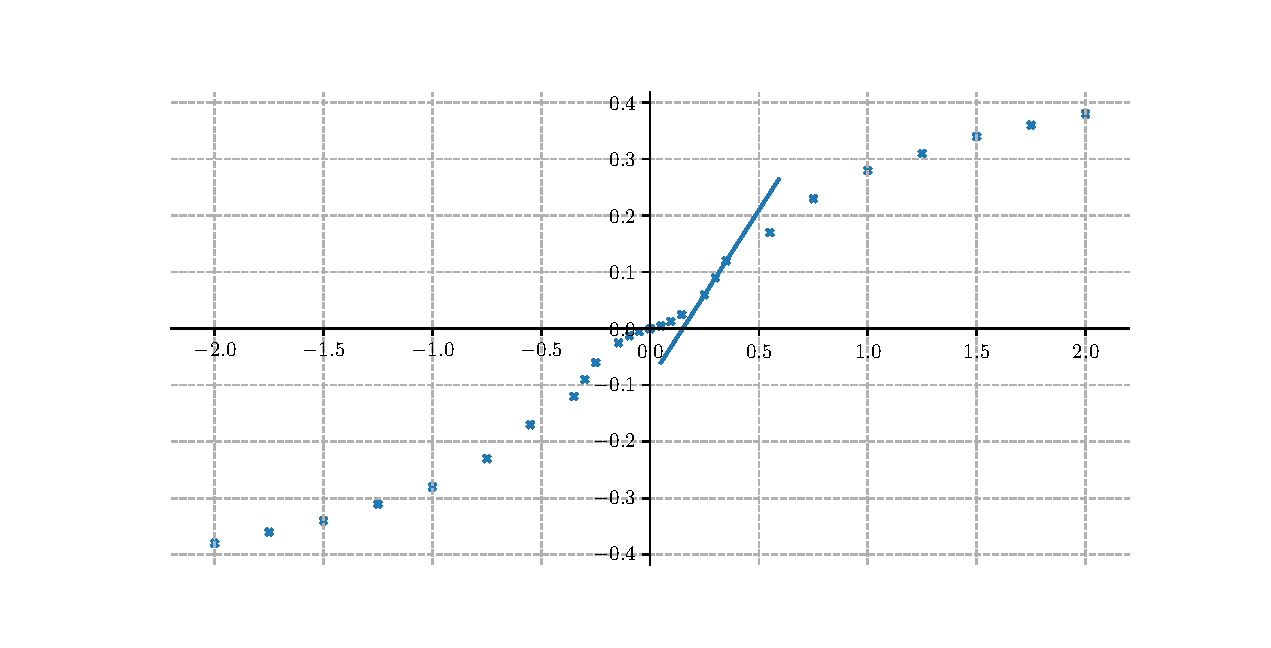
\includegraphics[width=0.9\linewidth]{pics/sife.eps}
    \text{(б) Кремнистое железо}
    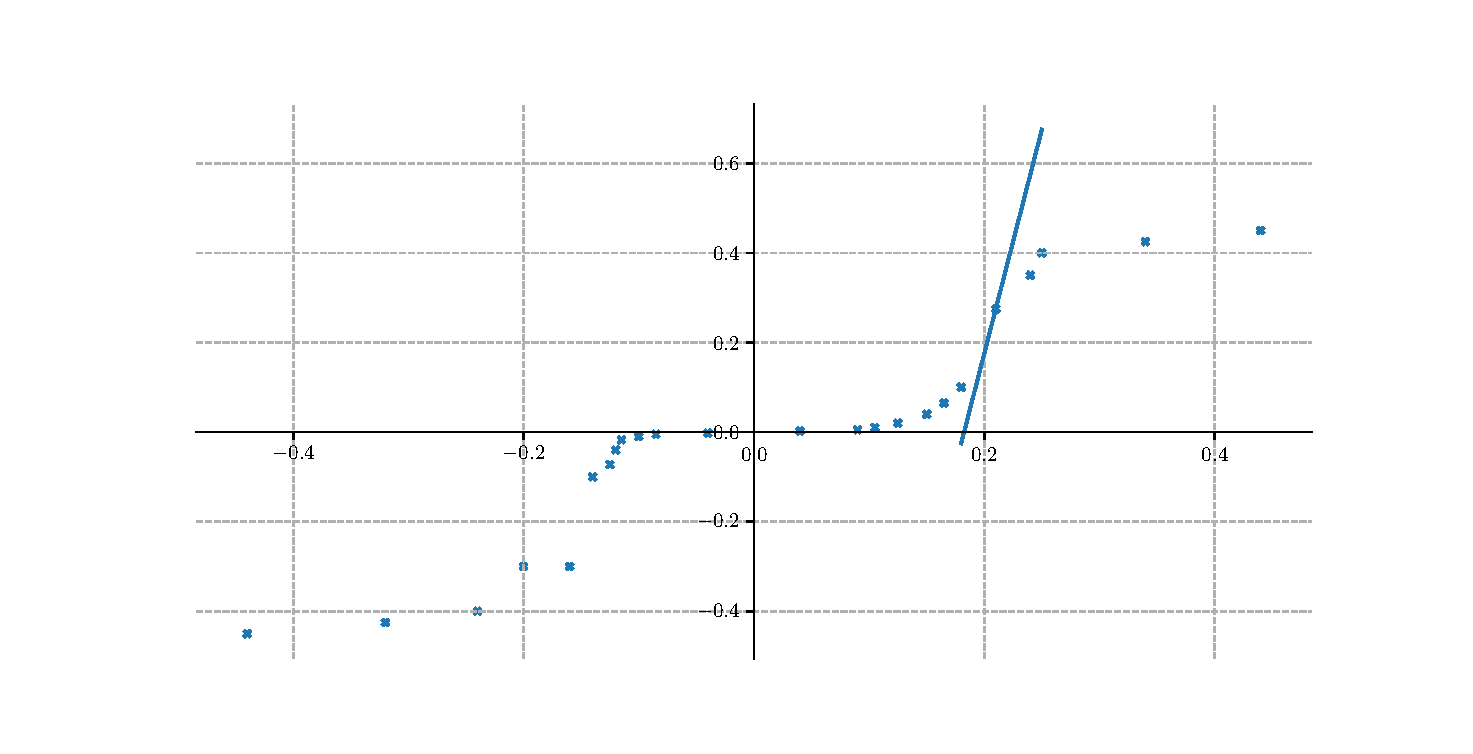
\includegraphics[width=0.9\linewidth]{pics/perm.eps}
    \text{(в) Пермаллой}

	\caption{Кривые намагничивания}
\end{figure}

По построенным кривым и предельным петлям гистерезиса определим некоторые параметры образцов (табл. 4)
\begin{table}[H]
    \centering
    \begin{tabular}[]{|l|c|c|c|}
        \hline
        &Феррит&Кремнистое железо&Пермаллой \\ \hline
        $H_c$, $\frac{А}{м}$ &18.0 &272.7&121.9\\ \hline
        $B_s$, Тл &0.35 &3.8&9.09 \\ \hline
        $B_r$, Тл &0.198 & 1.6&9.09 \\ \hline
        % $\mu_{max},\ 10^{-3}$  & 11 & 6.6 &223.3 \\ \hline
        $\mu_{max},\ 10^{3}$  & 8.8 & 5.3 & 177.7 \\ \hline
    \end{tabular}
    \caption{Параметры образцов}
\end{table}

Также расчитаем постоянную времени интегрирующей ячейки $\tau$ по формулам (4) через $R_и$ и $С_и$ и через напряжение, подобранное так, что $U_{вх} = 2y K_y$ (аналогично для $U_{вых}$).

$\tau_U \simeq 0.31\ Ом \cdot Ф,\quad \tau_{RC} \simeq 0.4\ Ом \cdot Ф$.

\subsection*{Подведение итогов}
В ходе работы проведена калибровка осей осциллографа, восстановлена начальная кривая намагничивания и по петлям гистерезиса для различных образцов установлены их свойства. 
Многие из них сильно разнятся с табличными значениями, что может свидетельствовать как о некачественных сплавах, так и о несовершенстве используемых для расчета методов.
\end{document}